\documentclass[12pt]{article}

\usepackage[english]{babel}
\usepackage[utf8x]{inputenc}
\usepackage{amsmath}
\usepackage{graphicx}
\usepackage{hyperref}
\usepackage{color}

\title{ECE 110 Final Lab Project}
\author{
  Bhargava Manja
  \and
  Robert McDonald
}

\begin{document}
\maketitle

\section{Introduction}
The goal of the ECE 110 final lab project is to design, implement, test, and
debug an autonomous vehicle that, using infrared sensors, can accurately follow
a track. Students had the option of designing and implementing a car that
utilized TTL circuit logic or one that used an Arduino micro controller. We decided to use an Arduino micro controller (specifically the Arduino Micro board) for
the sake of simplicity and ease. We were more familiar with the programming
concepts that an Arduino based design required. Using an Arduino and two H-bridges, we have successfully implemented an autonomous vehicle that follows a grid,
only turning when the car's sensors detect gray tape. The design also incorporates an element of state remembrance, as it correctly implements turns on T and cross intersections by ``remembering'' turn indicators placed several inches away
from such intersections.

\section{Documentation of Design}
\subsection*{Code}
You can see the latest version of our code at: \url{https://github.com/Bhargee/ece110/blob/master/ece110.ino}.
\subsection*{Circuitry}
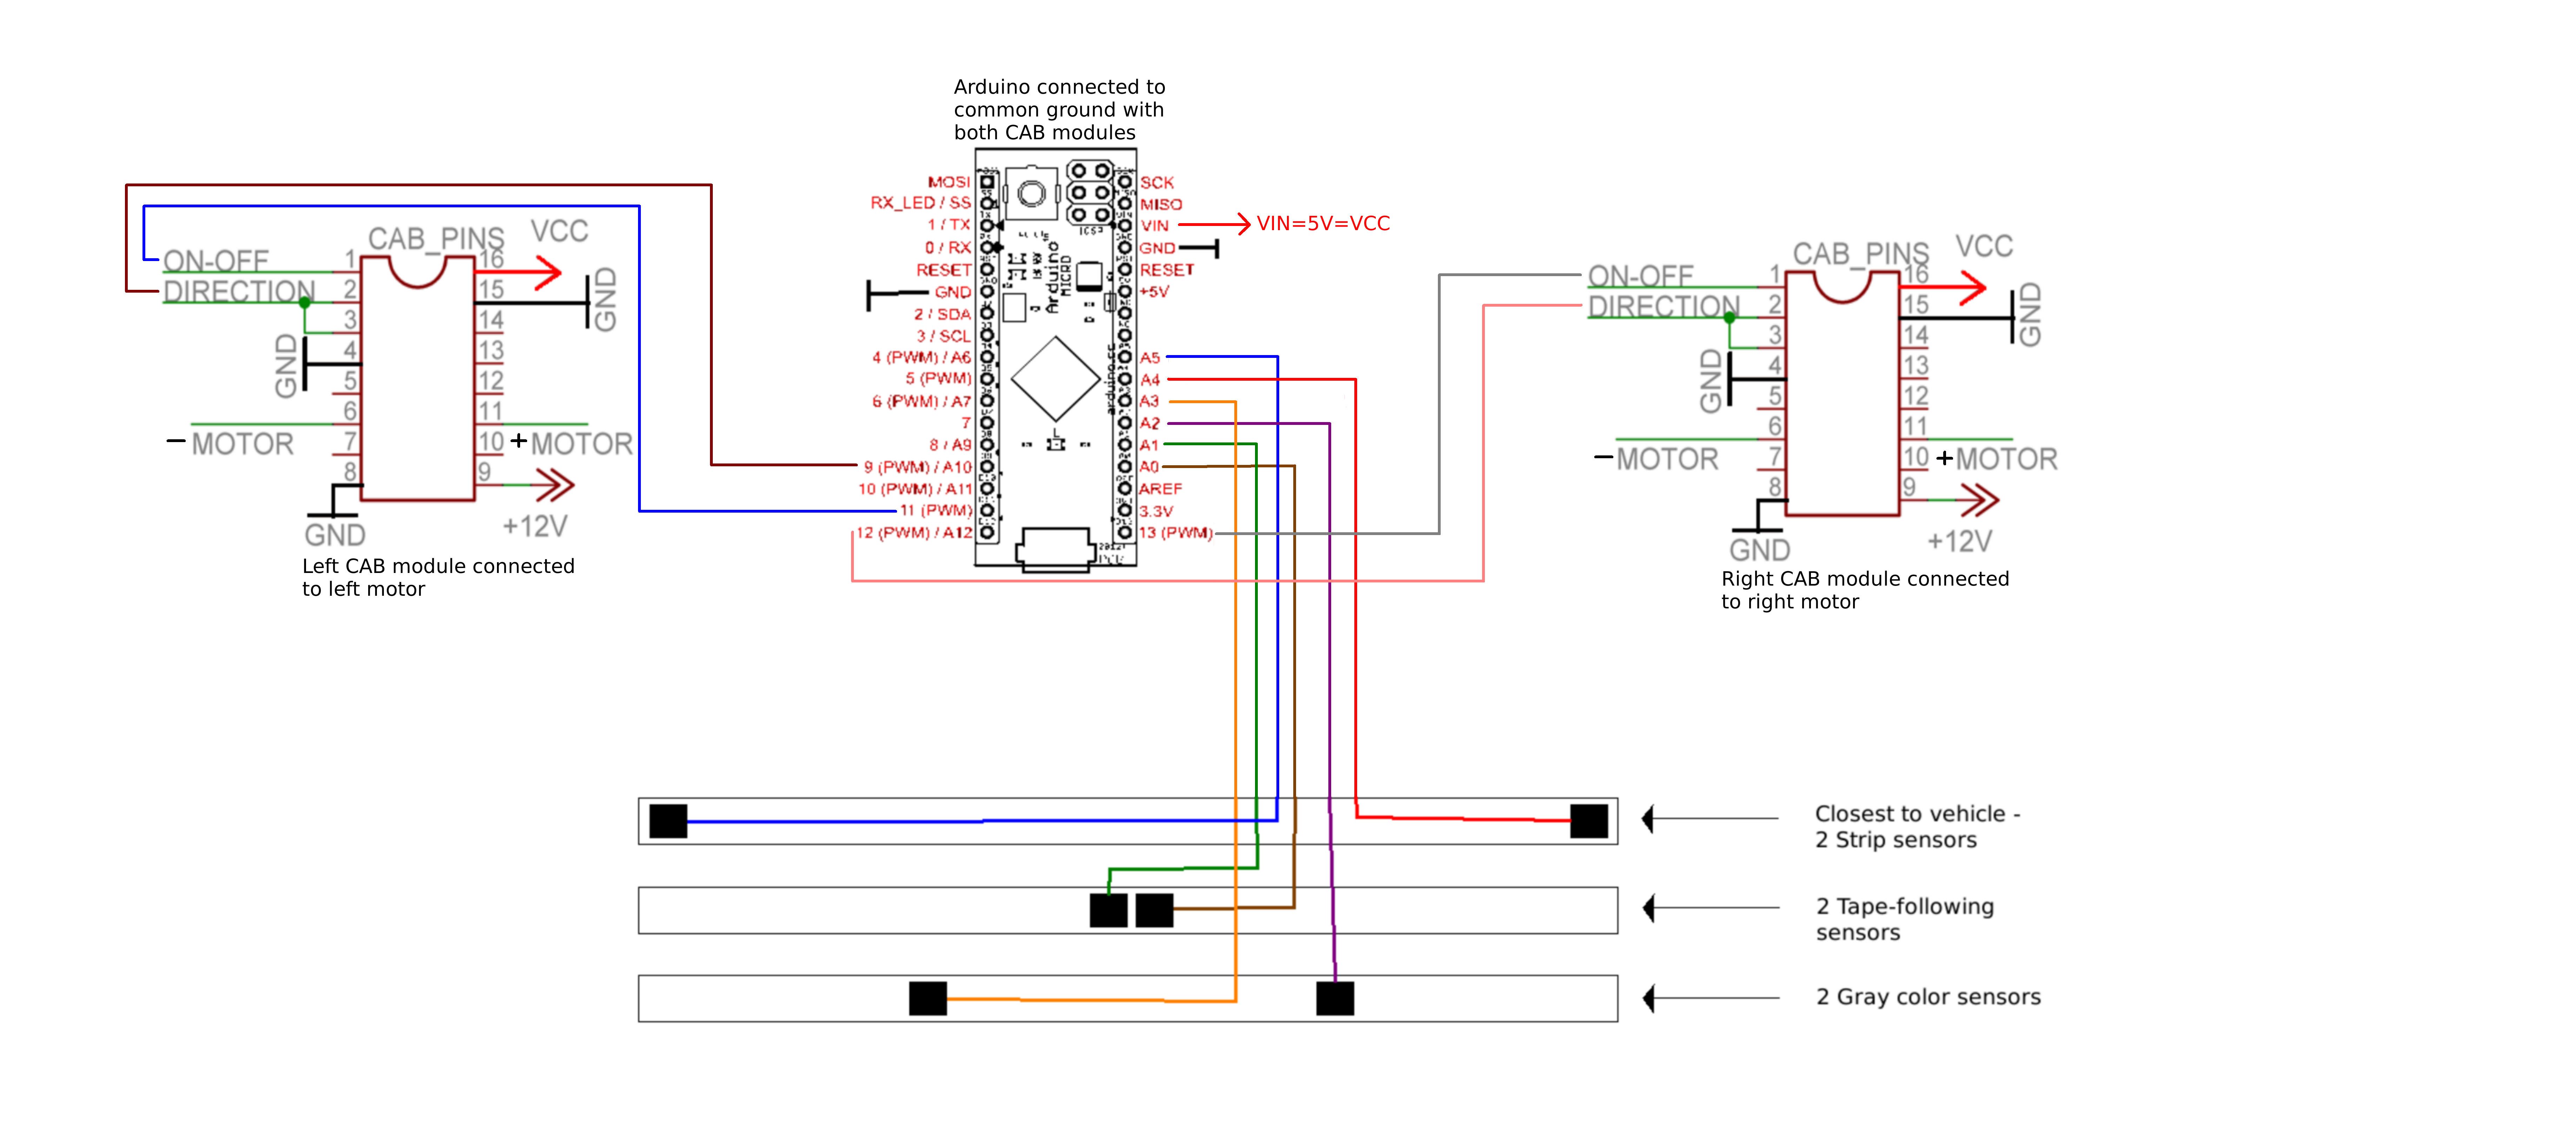
\includegraphics[scale=.10]{pinout.png}

The Arduino Micro allows us to program the car's logic so it responds to certain sensor inputs. This allows us to save a lot of space on the protoboard as well as eliminating wiring mistakes because we do not have to place nearly as many components on the board.

The CAB modules are used to control the direction the wheels turn on each side of the car. Our design utilizes these CAB modules so that we can execute 90 degree turns while keeping the center of the car in the same spot on the track. The other option would have been to stop one set of wheels and have the other set run forward, but we opted to use the former because the car does not have to move as far, so a bad turn is less likely to occur. 

The sensors give an analog signal to the Arduino, which then reads the values and then outputs a digital signal to each CAB module. The CAB modules then send the appropriate voltages to each respective motor. This effectively determines the direction each set of wheels turn. 

The sensor outputs are also used by the Arduino to determine the speed at which each set of wheels run. The Arduino does this by inputting the sensor outputs to a Pulse Width Modulator, which sends pulses of a high voltage to the motor. The amount of time these pulses last in comparison to how long the pulses are not occurring determines the speed of the motors. The longer the pulses are occurring compared to how long they are not occurring makes the motor go faster, and vice-versa. The PWM outputs go to each respective CAB module and then through the CAB modules to each respective motor. 

\section{Design Philosophy}
The choice of Arduino over circuit logic was easy for us. We were already
familiar with programming micro controllers, and we recognized from personal
experience that debugging an Arduino would be far easier than debugging a
circuit. We chose the Arduino Micro because it was one of the cheapest models
and because its pin out was the same as the Arduino Leonardo, so for the
negligible price we got a full fledged micro controller. One major advantage of
the Micro is that it plugs right into the protoboard, which makes wiring easier
and neater and eliminates an entire class of wiring problems.

\subsection*{Navigation Strategy}
Because of the nature of the Arduino car track, we realized that the tape
following scheme was the most hassle-free way of navigation, as tape avoiding,
the other possible scheme, would be thwarted by intersections. To deal with
keeping a straight path when there was a branch with the tape avoiding scheme, we would need to add code and sensors, which would add failure points. Thus making
the tape-following decision was simple. Tape following worked well enough that we
didn't need to make any adjustments to the sensor values in code. We simply read
the tape following sensor values, mapped the values from 10 bit to 8 bit, and
wrote the values straight to the motors. This choice came with some added benefits. It helped minimize the number of sensors we needed for detecting and making
right angle turns. The tape following sensors themselves could be used to detect
turns, as turns were marked with gray tape. Thus we only needed two additional
sensors to detect the direction of the turn based on the way the gray tape was
laid out. Tape following lent itself to simplicity of sensor layout and code.

\subsection*{Sensor Number}
Deciding the number of sensors was another easy decision. We needed a minimum of
two tape following sensors, which played double duty as part of our turn
detection system. We needed two more gray sensors to detect turn direction (on
either side of the car), and two sensors to detect the strips that signaled
turn direction on T and cross intersections. We found that more sensors were
unnecessary. The relatively small number of sensors helped with both code
and hardware debugging.

\subsection*{Sensor Layout}
Sensor layout was easily the most difficult part of this entire endeavor. We
originally had all the sensors on the same bar, but this design quickly ran into
trouble. We would calibrate the perceived ranges for black, white, and gray by
changing the height of the single sensor bar, but this careful calibration would
break down at turns, as the turn sensors would simply read the grays incorrectly,
and were often confused by the region where white crossed over to black. Thus, we
decided to split up our three sensor subsystems. We could calibrate each
individually, which gave us more room in setting our cutoff points in code and
greatly increased the accuracy of the gray sensors. We kept all the sensors close
to the car body so they wouldn't accidentally read wrong parts of the track, as the 
car is quite large relative to the size of the track. The tape following and
strip sensing sensors were the closest for the purpose of accuracy. The gray
sensors, which told the micro controller which way to turn, were in the middle
sensor bar rack, as the tape on the turning parts of the track was set up so that
the actual turn was several inches before the gray tape started. Thus we could afford to keep the directional sensors in front. Spacing them out also allowed
the car to accurately detect when to stop turning, so we didn't have to rely
on timing turns, which is prone to error
. In code, we programmed
turns to stop when the tape following sensors were white (the path) and the
turn detection sensors see black (just off the path). We played with the
distances between the two sensor bars so the car would stop consistently at the
right place. This distance happened to be two sensor rack locations away.

\subsection*{Code}
The code implements a simple Finite State Machine with entry conditions. We had
to break the ``purity'' of the FSM because of the real world concern of things
not working properly. Whenever we needed to put in a hack to get the car to work
(which was often), we had to break, at least partially, the FSM model. We defined
four states with \verb|enum robot_op = {normal, cw, ccw, halt}|. This enum
defined our normal navigational state, our clockwise and counterclockwise turn
state, and our stopped state. In \verb|void loop()| the actions that change the
state of the FSM are sensor inputs, for example, when \verb|if(state == normal && is_grey(l_tape_follow) && is_grey(r_tape_follow))|, then the state changes to a
turning state depending on some variable values and more sensor checking. The
only real hack is turning, which uses a while loop and has two methods of
termination. It uses a counter, but will stop the turn when the tape following
sensors see white and one of the turn detection sensors see black. This worked
extremely well for us in testing. We also included a debug mode variable that
simply returned from the loop after printing out sensor values when true. The
turning code breaks the FSM paradigm, but works just as well when it is a proper
part of the state machine. We haven't changed the code back as it would differ from the code we uploaded on the Arduino.

\section{Results}
Our entire navigation scheme worked very well on a smaller version of the track we made. It was made out of a large black posterboard and we applied white tape and gray paper to complete the track. The tape following scheme worked very well and was even able to find its way back onto the white tape when it was far away due to the implementation of the PWM in the coding. The gray color detection worked very well also. This was a problem for us early on due to an inability to differentiate between white and gray by any significant amount. We originally had one sensor bar with all six sensors on it, but we found that we could not find a sensor bar height that would allow us to get readings within the desired ranges. To fix this issue, we decided to implement more sensor bars. Then we were able to calibrate our sensors much more effectively and consistently. After we decided to use more sensor bars, our gray detection was perfect.

Between our coding and sensor detection, the car was able to consistently navigate the 90 degree left and right turns. Our strip detection turns were the only turns that were not near perfect. We were able to read a left strip and turn left at the intersection as well as read a right strip and turn right at the intersection consistently, but we were never able to read both strips and continue going straight. This was probably an error in the code.

On the day we officially tested the car, however, things did not go so well. We are confident that the difference in performance was due to the sensors, lighting, or sensor bars. We know that all of the sensors were getting correct readings when calibrated, but for some reason, the car did not execute the expected functions. We know that the sensors were reading gray at seemingly random times because we were able to review the values after an attempted run. This completely undermined our navigation scheme because the sensing of gray can mean a lot of different things depending on which sensors see them. This is why our car would not properly execute turns and also why it would turn at random times. We are confident that the difference in reflectivity between the black surface of the test track and the track we made caused the sensors to see gray at the point where the white tape met the black surface. The difference in lighting conditions also played a key role in this anomaly. Thus, our results are ambiguous. Our design worked almost
perfectly on our test track, yet broke down (like the other Arduino cars) on the
real track because of issues with mistaking white and black for gray.
\section{Future Work}
To be honest, we would not change much if we could start over. The hardware setup
was optimal, as we had minimal wiring, a small number of sensors, and a small
footprint on the protoboard. The code is simple and intuitive. One thing that
never properly worked was strip detection for the T intersections. We would
probably separate that logic from the normal turn logic in code, as the issue
with the scheme was that the T intersections would be often mistaken for normal
turns. If we had more time, we would have tried to mitigate the effects of
different lighting conditions/tracks, as our performance varied widely between
the test tracks (both our own and the one on the final day) and the actual track.
We did not think that would be an issue, but it turned out to be a huge problem.
We should have checked against different track conditions and tried to come up
with an automated or programmatic way of dealing with bad conditions. Other than
that, we are fully satisfied with our design.

\section{Conclusion}
Overall, I think this was a very beneficial learning experience. We learned many things in the lab as well as working on the project on our own. It was a time-consuming, but very worthwhile project in which we learned about the actual implementation of the devices we learned about in lecture. This definitely solidified in our minds some of the concepts that we have learned in lecture. Some of the devices, such as the multiplexer, for example, make much more sense when implemented in the lab with live inputs that are constantly changing to the tables of variables at given times that we are tested on. This is the reason why our experience in the lab is so critical to the total understanding of what we have learned about in ECE 110. In addition, we now have experience with the Arduino and micro controller programming, which is invaluable. This project was a great preparation for future classes, as we have actually implemented and debugged what we learned about in lecture.

\end{document}
